% --- OSI


\tabsec{Problemstellungen auf Bitübertragung \& Sicherungsschicht:}
\begin{tabbing}
Problem \= Zuverlässige Zustellungenen \= Spalte 3  \kill
\> Kodierung:	\> Kodierung von Bits	\\
\> Framing:		\> Zusammenfassen von Bits in Frames	\\
\> Fehlererkennung: \> Bitfehler erkennen	\\
\> Zuverlässige Zustellung: \> Empfang sicherstellen (trotz Fehlern)	\\
\> Medienzugriff: \> Reihenfolge der Sender regeln	
\end{tabbing}

\Minisec{Problemstellung auf Transportschicht}
Garantierte Übertragung, beibehalten der Reihenfolge, Beliebige Nachrichtengrößen, \\
Adressierung mehrerer Anwendungsprozesse, Flusskontrolle, Überlastkontrolle

% --- Schicht 1
\tabsec{Betriebsweisen:}
\begin{tabbing}
Richtungen: : \= Simplex mit Quittungen  \=  \kill
"Taktung":\> Synchron : \> Zentraler Takt\\
	\> Asynchron: \> Senden zu beliebigen Zeitpunkten\\
"Richtungen":\> Simplex : \> Eine Richtung	\\
	\> Simplex mit Quittung: \> Eine Richtung, ACKs in Gegenrichtung\\
	\> Halbduplex : \> Abwechselndes Senden	\\	
	\> Vollduplex : \> Senden in beide Richtungen	
\end{tabbing}


\tabsec{Modulation:}
\begin{tabbing}
Amplitudenmodulation : \= Kodieren in verschiedenen Signalpegel (z.B.0V, $\pm$ 5V, \dots)\\
Frequenzmodulation : \> Kodieren in verschiedenen Frequenzen \\
Phasenmodulation : \> Kodieren in Phasensprüngen (z.B. Richtungswechsel in Sinuskurve)	
\end{tabbing}


% --- Schicht 2
\Minisec{Frame-Varianten:}
\textbf{Byte-Zähl-Methode:} Längenangabe in dezidiertem Feld\\
\textbf{Sentinel-Methode:} Frame wird durch Sentinel-Zeichen strukturiert: STX (Start of Text), ETX (End of Text), DLE (Zeichen-Excape)
ETX und DLE müssen im Nutzdatenteil durch DLE escaped werden. (Zeichenstopfen)

\Minisec{Fehlererkennung:}
\minisec{Eindimensionale Parität:}
Einfügen eines Zusatzbits (Gerade Parität = Anzahl aller 1Bits gerade)


\minisec{2-dimensionale Parität:}
Eindimensionale Dimensionalität + Einfügen einer Zeile mit Parität über die Spalten, z.B.:
\begin{tabular}{|cccc|c|}
\hline
0 & 1 & 0 & 1 & 0 \\
1 & 1 & 1 & 0 & 1 \\
\hline 
1 & 0 & 1 & 1 & 1 \\
\hline
\end{tabular}


\Minisec{ARQ (Automatic Repeat Request)}
Empfänger: Frame korrekt empfangen : sende ACK \\
Sender: Wenn kein Ack innerhalb Timeout : Frame neu senden \\
Frame beinhaltet Sequenznummer;

\minisec{Stop-and-wait}
immer nur ein Frame unterwegs;

\minisec{Sliding-Window}
Sender: ZuletztGesendet - LetztesAck $\leq$ SendeFenstergröße\\
Empfänger: MaximalesACK = LetzterFramevorLücke + EmpfangsFensterGröße

\minisec{ACKS:}
\begin{itemize}
\item Kumulativ: Letzter Frame vor Lücke, z.B. Empfangen: 1,2,3,7 => ACK(3)
\item Selektiv: Empfangene Frames werden bestätigt: z.B. Empfangen 1,2,3,7 => ACK(1,2,3,7)
\item Negativ: Fehlende Frames werden übermittelt: z.B.b Empfangen 1,2,3,5 => NAK(4)
\end{itemize}
Duplicate ACKs: Wenn ein kumulatives ACK doppelt => Nachsenden des darauf folgenden Frames (nur 1x pro Timeout)



\Minisec{Medienzugriff}
CSMA/CD(Ethernet): Sender Erkennen Kollisionen
\begin{itemize}
\item Medium frei: sende
\item Medium nicht frei: sende nicht
\item Kollision erkannt: senden abbrechen \& Stausignal
\item Exponential Backoff: wähle Zufallszahl z aus {0,$cdots, 2^n-1$} mit n = anzahl Kollisionen; warte z * 51,2 $\mu$
\end{itemize}

CSMA/CA(WLAN): Erkennung nicht möglich => Kollisionsvermeidung
\begin{itemize}
\item Medium frei: sende
\item Medium nicht frei: warte bis Medium frei + zusätzliche Wartezeit\\
Wartezeit = DIFS + zufällige Wartezeit \\
Wartezeit für ACKS = SIFS (priorisierte Behandlung)
\end{itemize}

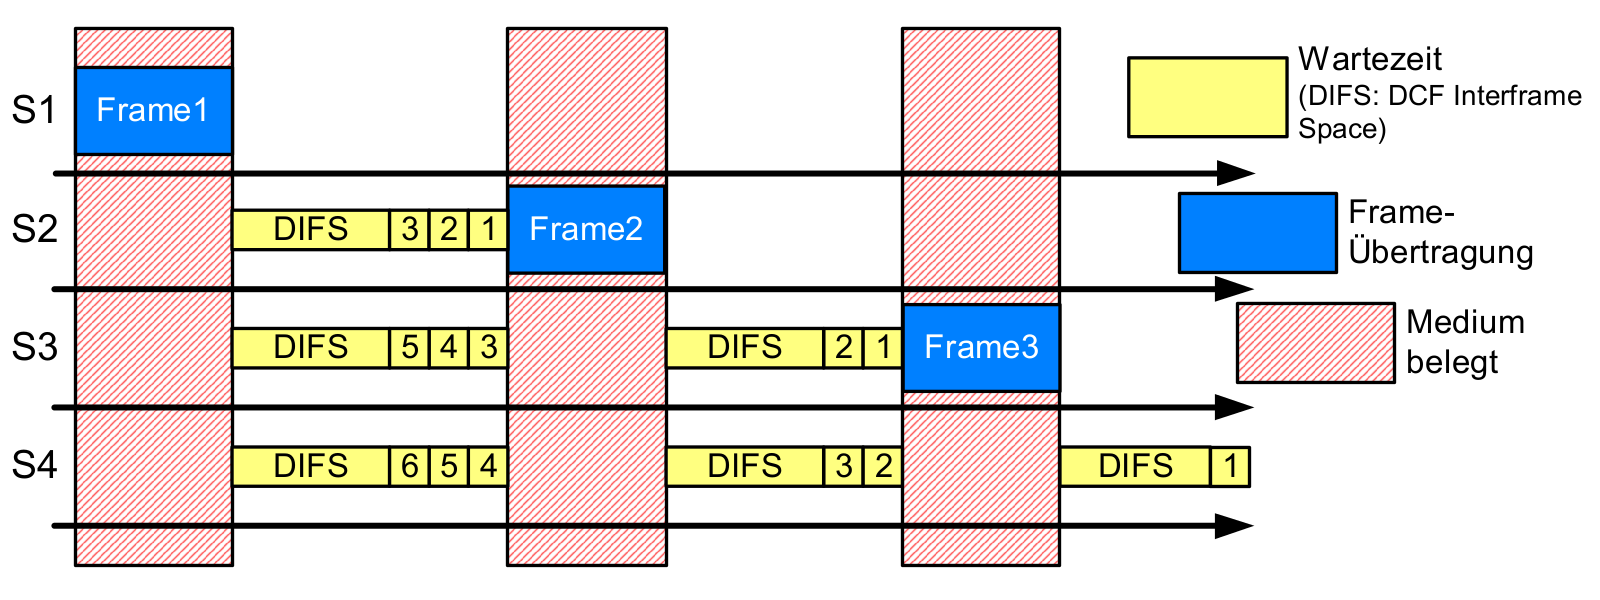
\includegraphics[width=0.5\textwidth]{CSMA-CA}




Master/Slave: Ein Teilnehmer erteilt Senderecht an untergeordnete Slaves

Token Ring: Bitmuster (Token) repräsentiert Sendeberechtigung

% --- Schicht 3
\Minisec{Routing}
VLANs: Trennung von Subnetzen auf Switch-Ebene\\
Packet Switching: Jedes Packet wird einzeln gerouted (kein Verbindungsaufbau)\\
Circuit Switching: Routingentscheidung am Anfang der Verbindung\\
Source Routing: Sender berechnet Route und schreibt sie ins Paket beinhaltet die Route

\Minisec{Link-State-Routing}
Ermitteln der Distanz zu den Nachbarn, Informationsweitergabe an alle Knoten (Fluten)\\
Jeder Knoten berechnet Netzwerktopologie und daraus den kürzesten Weg => Dijkstra\\


\minisec{Fluten}
Jeder Knoten sendet Link-State-Pakete an alle Nachbarn \\
Optimierung: kein zurückschicken, doppelte Pakete verwerfen, TTL, MPR(siehe OLSR)


\Minisec{Distance-Vector-Routing}
Ermitteln der Distanz zu allen Knoten, Informationsweitergabe an die Nachbarn


\minisec{Zuweisung:}
\begin{minipage}{0.5\textwidth}
\begin{itemize}
\item Stateful: über DHCPv6
\item Autoconfiguration: 
\begin{enumerate}
\item Berechne Identifier (aus MAC oder zufällig)
\item => frage bei Router mit fe801::/64 + Identifyer (Link Local Unicast Adresse)
\item Router teilt mögliche Präfixe mit
\item Host prüft ob Adresse schon vorhanden (Double Address Detection)
\end{enumerate}
\end{itemize}
\end{minipage}


\Minisec{DHCP:}
\begin{enumerate}
\item Client: DHCPDISCOVER (per Broadcast)
\item Server: DHCPOFFER 
\item Client: DHCPREQUEST
\item Server: DHCPACK (Client hat nun Adresse geleast)
\end{enumerate}
Erneuerung des Leases (DHCPREQUEST) nach 50\%-87,5\% Leasezeit, danach nur über DCHPDISCOVER


ICMP: Fehlernachrichten von IP
ARP/NDP: Auflösen von IP in MAC-Adressen in IPv4/v6	\\
Bei NDP auch Router-Advertisements: Router sendet Präfixe per Broadcast.

% --- Schicht 4 
Pseudo-Header: enthält Felder aus IP-Header (v.A. Adressen) für Prüfsumme\\
Aufbau: 3-way Handshake, \\
Abbau: 3-way-Handshake oder 4-way-Handshake(halboffene Verbindung)

Sender verwaltet: MaxSendePuffer, LastByteSent, LastByteAcked\\
Empfänger verwaltet: MaxEmpfangsPuffer, lastByteRead, nächstes Fehlendes Byte, lastByteRecieved

\\
Für Effective Window (siehe Sliding Window): verwende CongestionWindow statt AdvertisedWindow wenn dieses kleiner


\minisec{Duplicate Acks / Fast Retransmission}
Bei 3x gleiches ACK: Folgendes Paket neu senden (vgl. Duplicate Acks Schicht 2) Grund: Umordnung möglich



% --- P2P
\textcolor{green}{Skalierbarkeit, Ausfallsicherheit, Kosten,} \textcolor{red}{Überwachung, Administrierbarkeit, Kommerzieller Einsatz}

\minisec{Distributed Hashtable:}
Hashtable: Zuordung Hashwert(Suchanfrage) zu Zieladresse; wird auf Peers verteilt;




% --- Sicherheit

Firewall: Router mit Paketfilter 

rekursiv(1): Gefragter Nameserver besorgt die richtige antwort (lokale NS)\\
iterativ(2-4): gefragter Nameserver schlägt tieferliegenden Nameserver vor\\
autoritativ(5): vollständige Antwort (Wenn Adresse bekannt)\\


